\chapter{Backend Mystery} 

\section{MTV Framework}
The apps are modularized. You can remove your  application by deleting one directory instead of hunting through several directories deleting each piece. 

\begin{figure}[htb]
\centering
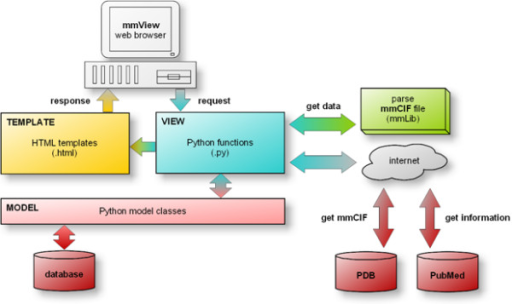
\includegraphics[scale=0.6]{./mtv}
\caption{Django MTV framwork(cite from internet)}
\label{fig:label} % insert suitable label, this is used to refer to a fig from within the text as shown above
\end{figure}
\textbf{M} represents the model (Model), i.e. the data access layer. The layer processing and data in all matters related to: how to access, how to confirm the validity of including which the relationship between behavior and data.\\
\textbf{T} Representative of T template (Template), i.e., the presentation layer. The layer processing performance related decision: how to display the page or other types of documents.\\
\textbf{V} represents the view (View), business logic layer. This layer contains the access models and the transfer of appropriate template logic. You can see it as a bridge between the model and the template.\\
\section{Models and Database}
Django provides an abstraction layer (the “models”) for structuring and manipulating the data of your Web application. \\
In Django, a lot of this hassle is taken care of for you by Django’s object relational mapping (ORM) functions, and how Django encapsulates databases tables through models. Essentially, a model is a Python object that describes your data model/table. Instead of directly working on the database table via SQL, all you have to do is manipulate the corresponding Python object. 
\section{Django Template Language}
Django’s template language is designed to strike a balance between power and ease. It’s designed to feel comfortable to those used to working with HTML. \\
Django template language is not just HTML file. Here is an example:
\begin{verbatim}

<nav id="navigation">

    <ul class="book-page-list">
    
    
    <li><a href="{{ page.get_absolute_url }}">{{ page.name }}
    
        <li class="active">{{ page.name }}</li>
    
    
    </ul>

</nav>

\end{verbatim}

Variable A {{a}}
Tag b 
c filter d{{c|d}}

we can add variables tags and filters into html code.

\section{Request-Response Flow}

How Teakwood process a request from user?
\begin{figure}[htb]
\centering
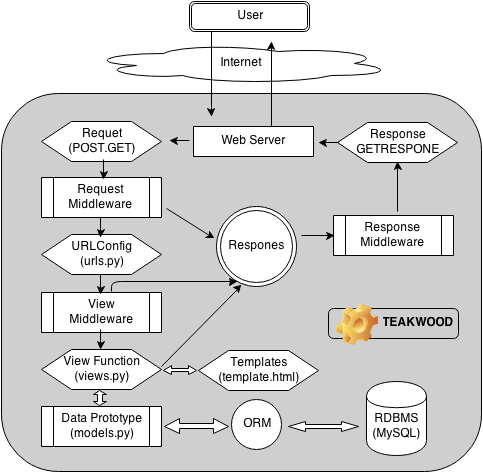
\includegraphics[scale=0.6]{./http_request_response}
\caption{<Caption here>}
\label{fig:label} % insert suitable label, this is used to refer to a fig from within the text as shown above
\end{figure}

%\section{Lose Coupling}
\section{Powerful Admin}
Django comes with a user authentication system. It handles user accounts, groups, permissions and cookie-based user sessions. This section of the documentation explains how the default implementation works out of the box, as well as how to extend and customize it to suit your project’s needs.

